\documentclass[a4paper, 11pt]{article} % Font size (can be 10pt, 11pt or 12pt) and paper size (remove a4paper for US letter paper)

\usepackage[protrusion=true,expansion=true]{microtype} % Better typography
\usepackage{graphicx} % Required for including pictures
\usepackage{wrapfig} % Allows in-line images
\usepackage{mathpazo} % Use the Palatino font
\usepackage[T1]{fontenc} % Required for accented characters
\usepackage{amscd,amsmath}
\usepackage{tikz,stmaryrd}
\usepackage{latexsym,amsbsy,bbold, fullpage}
\usepackage{amssymb,amsthm,amsfonts}
\usepackage{pdfsync,yfonts}
\usepackage{tkz-graph}
\usepackage[all,pdf]{xy}
\usepackage{ctex}  %支持中文

%\usepackage[BoldFont,SlantFont,CJKchecksingle,CJKnumber]{xeCJK} %设置中文
%\setCJKmainfont{SimHei} %黑体
%\setCJKmonofont{Monaco} %设置缺省中文字体
%\usepackage{CJK}


%%%%%%%%%%%%%%%%%%%%%%%%%交换图示例%%%%%%%%%%%%%%%%%%%%%%%%%%%%%%%%%%%%%%%%%%

%$$\xymatrix{
%\widetilde{K}(S(X\times Y))\ar[r]^{Si^*}
%&\widetilde{K}(S(X\vee Y))\ar[r]^{\delta}\ar[d]^{\cong}_{S\alpha}
%&\widetilde{K}(X\wedge Y)\ar[r]^{p^*}
%&\widetilde{K}(X\times Y)\ar[r]^{i^*}
%&\widetilde{K}(X\vee Y)\ar[d]^{\cong}_{\alpha}\\
%&\widetilde{K}(SX)\oplus \widetilde{K}(SY)\ar @{.>}[ul]^{S\eta}&&
%&\widetilde{K}(X)\oplus \widetilde{K}(Y)\ar @{.>}[ul]^{\eta}
%}$$

%%%%%%%%%%%_________The following are examples of pictures__________%%%%%%%%%


%\begin{figure}[ht]
%\centering
%\includegraphics[width=0.2\textwidth]{kdd.png}
%\caption{kuntion}
%\end{figure}

%%%%%%%%%%%%%%%%%%插入表格示意%%%%%%%%%%%%%%%%%%%%%%%%%%%%%%%%%%%%%%%%%%%%%%%%
%$$\begin{tabular}{|c|c|c|}   % |:竖线, l、c、r := 居左,居中,居右
%\hline
%直角边$a$ & 直角边$b$ & 斜边 $c$\\
%\hline
%3 & 4 & 5 \\
%\hline
%5 & 12 & 13 \\
%\hline
%7&24&25$\frac{1}{2\pi\sin\theta}$\\
%\hline
%\end{tabular}$$
%%%%%%%%%%%%%%%%%%%%%%%%%%%%%%%%%%%%%%%%%%%%%%%%%%%%%%%%%%%%%%%%%%%%%%%%%%%%%%%

\newcommand*{\vs}{\vspace{5pt}}
\newcommand*{\vsp}{\vspace{10pt}}
\newcommand*{\vspp}{\vspace{15pt}}
\newcommand*{\kong}{$\,\,\,\,\,\,\,$}
\newcommand*{\ad}{\text{ad}}

%\newcommand*{\ad}{\text{ad}}
\newcommand*{\Der}{\text{Der}}
\newcommand*{\ra}{\rightarrow}

\newcommand*{\defn}{\textit{Definition}:}
\newcommand*{\rmk}{\textit{Remark}:}
\newcommand*{\Example}{\textit{Example}}

\newcommand*{\R}{\mathbb{R}}
\newcommand*{\C}{\mathbb{C}}
\newcommand*{\p}{\partial}
\newcommand*{\ten}{\otimes}

\newcommand*{\kai}{\CJKfamily{kai}}
\newcommand*{\hei}{\CJKfamily{hei}}
\newcommand*{\fs}{\CJKfamily{fs}}
\newcommand*{\song}{\CJKfamily{song}}

%%%%%%%%%%%%%%定理环境%%%%%%%%%%%%%%%%%%%%%%%

\newtheorem{thm}{定理}[subsection]
\newtheorem{prop}{性质}[subsection]
\newtheorem{definition}{定义}[subsection]
\newtheorem{example}{例子}[subsection]
\newtheorem{rem}{注记}[subsection]
\newtheorem{cor}{推论}[subsection]
\newtheorem{claim}{断言}[subsection]
\newtheorem{intro}{导引}[subsection]
\newtheorem{prob}{Problem}[subsection]


%%%%%%%%%%%%%%%%%%%%%%%%%%%%%%%%%%%%%%%%%%%%%%%%

\linespread{1.2} % Change line spacing here, Palatino benefits from a slight increase by default

\makeatletter
%\renewcommand\@biblabel[1]{\textbf{#1.}} % Change the square brackets for each bibliography item from '[1]' to '1.'
\renewcommand{\@listI}{\itemsep=0pt} % Reduce the space between items in the itemize and enumerate environments and the bibliography

\renewcommand{\maketitle}{ % Customize the title - do not edit title and author name here, see the TITLE block below
\begin{center} % Right align 可以换成 “flushleft”
{\Huge\@title} % Increase the font size of the title

\vspace{30pt} % Some vertical space between the title and author name

{\Large\@author} % Author name
\\\@date % Date

\vspace{20pt} % Some vertical space between the author block and abstract
\end{center}
}


\title{\textbf{曲豆豆的高等数学入门教程}\\$\,$\\% Title
卷一:基础架构} % Subtitle

\author{\textsc{曲豆豆\,\,\,主编} % Author
\\{\textit{豆瓣研究生小组\,\,\,\,\,荣誉出品}}} % Institution

\date{2018年12月4日\\
第02-3稿} % Date

%----------------------------------------------------------------------------------------
\begin{document}

\maketitle

%\renewcommand{\abstractname}{Summary} % Uncomment to change the name of the abstract to something else

\begin{abstract}
本讲义介绍近代数学的基本语言、架构,
包括朴素集合论与逻辑、基本的代数与拓扑结构,以及一元分析学。
\end{abstract}

\tableofcontents
\newpage
\chapter*{前言}
\addcontentsline{toc}{chapter}{前言}

近代数学的一个特点是公理化、结构化。
代表近代数学的布尔巴基(Bourbaki)学派认为“数学是研究抽象结构的学科”,
这与恩格斯的观点“数学是关于现实世界数量关系和空间形式的科学”略有出入。
本讲义力图介绍近代数学中的四大基本结构:序结构、代数结构、拓扑结构、测度结构,
从而勾勒出近代数学基本框架,满足那些“想要多学一些数学”的爱好者们的基本需求,
并为其进一步学习近代数学奠定基础。

虽说声称是“零基础入门高等数学”,
本讲义其实并不是真正的“白手起家”,
还是要假定读者对一些基本的数学对象有直观的了解,
包括:实数的加减乘除运算、实数大小的比较,仅此而已。

事实上,近代数学基础完整的构建顺序大概是:命题逻辑$\rightarrow$
一阶谓词逻辑$\rightarrow$公理集合论$\rightarrow$自然数公理系统
$\rightarrow$实数理论。什么是自然数中的“0”,什么是“1”,
“自然数”是在集合论的框架下定义出来的,并不是“本来就有的”;
而自然数的加法运算也是定义出来的,
不再是初等数学那样子来源于日常生活经验,理所当然的。
这也是为什么罗素用了300多页才得到了自然数“1”的定义,这才是真正的“白手起家”。
有了自然数,之后再定义整数,
通过对整数环分式化来构造有理数,
再对有理数完备化来构造实数。

而本讲义跳过这个漫长的构建过程(但会在正文各处穿插地简要提一下),
直接假定读者知道什么是实数,以及实数的加减乘除、大小比较。
这样做的原因有两点,其一是避免讲义篇幅过长,
过分纠结于数学基础是枯燥乏味的,毕竟这个讲义不是专门的“数学基础”教材。
其二是为我们要介绍的抽象结构提供具体例子,比如讲到“偏序集”这个结构时,
实数配以通常的比较大小就是一个例子;
讲到“群”结构时,实数配以加法运算就是一个最基本的例子。
离开具体例子空谈抽象概念并不利于对数学概念的理解(当然格罗滕迪克Grothendieck是例外)。

由于这个讲义是笔者写着玩的,
且笔者水平有限,胡说八道之处在所难免。
希望读者批判性地看待本讲义中的某些论断。
另外由于匆忙成稿,笔误、语法错误应该也挺多的,
恳请批评指正。

最后,关于自然数的公理化构造,笔者恶搞《圣经:创世纪》中的一段,仅供娱乐,见下页。
\newpage

\textbf{致谢}

感谢笔者母校中国科学技术大学数学系的培养

感谢豆瓣小组提供平台

感谢一起编纂此讲义的小伙伴们

\vspp
\textbf{贡献者(豆瓣昵称,按拼音字母顺序排序)}

曲豆豆,王有为,在云上,子坚

\begin{centering}
\newcounter{density}
\setcounter{density}{0}
\begin{tikzpicture}
    \def\couleur{green}
    \path[coordinate] (0,0)  coordinate(A)
                ++( 144:6cm) coordinate(B)
                ++(72:6cm) coordinate(C)
                ++(0:6cm) coordinate(D)
                ++(-72:6cm) coordinate(E)
                                ;
    \draw[fill=\couleur!\thedensity] (A) -- (B) -- (C) --(D) -- (E) --  cycle;
    \foreach \x in {1,...,120}{%
        \pgfmathsetcounter{density}{\thedensity+5}
        \setcounter{density}{\thedensity}
        \path[coordinate] coordinate(X) at (A){};
        \path[coordinate] (A) -- (B) coordinate[pos=.05](A)
                            -- (C) coordinate[pos=.05](B)
                            -- (D) coordinate[pos=.05](C)
                            -- (E) coordinate[pos=.05](D)
                             -- (X) coordinate[pos=.05](E);
        \draw[fill=\couleur!\thedensity] (A)--(B)--(C)-- (D) --(E)  -- cycle;
    }
\end{tikzpicture}

\end{centering}
\begin{centering}

\tikzstyle{level 1}=[sibling angle=120]
\tikzstyle{level 2}=[sibling angle=60]
\tikzstyle{level 3}=[sibling angle=30]
\tikzstyle{every node}=[fill]
\tikzstyle{edge from parent}=[snake=expanding waves,segment length=1mm,
                              segment angle=10,draw]
\begin{tikzpicture}[grow cyclic,shape=circle,very thick,level distance=13mm,
                    cap=round]
\node {} child [color=\A] foreach \A in {red,green,blue}
    { node {} child [color=\A!50!\B] foreach \B in {red,green,blue}
        { node {} child [color=\A!50!\B!50!\C] foreach \C in {black,gray,white}
            { node {} }
        }
    };
\end{tikzpicture}
\end{centering}

\newpage

\begin{centering}
\begin{Large}
\textbf{《圣经:创世纪》节选}
\end{Large}\vsp
\large

起初,神创造逻辑。

逻辑是空虚的。

神的零运行在水面上,

这是平凡的。

神说,要有集合。

于是就有了集合。

神看集合是好的,

就将其公理化。

有集合,有运算,

就是一个代数结构。\vsp

神照自己的样子造人,

于是就有了0.

神在东方的伊甸建立了一个园子,

称之为群。

神将0安置在那里,

让它作幺元。

起初,伊甸园是平凡的。

神说,园中所有果子你可以随便吃。

只有后继树上果子,你不能吃。

因为你吃的时候必死。\vsp

神说,那人独居不好。

于是要为它造一个配偶。

神让0沉睡,取它的后继数1.

神把1带到伊甸园,

让它和0配对,

二人从此一起生活。

神教给它们加法的运算,

让它们可以互相交合。

0依然是伊甸园的单位元。

0的逆元是0,1的逆元是1,

0和1彼此交合则又得到1.\vsp

神所造的,

惟有皮亚诺比一切的活物更狡猾。

皮亚诺对1说,

神岂是真说不许你们吃园中所有树上的果子么?

1对皮亚诺说,

园中树上的果子我们可以吃,

唯有后继树上的果子不可,

免得我们死。

皮亚诺说,你们不会死。

神是怕你们吃了后继树上的果子,

能自己创造新的数。\vsp

皮亚诺告诉1它自己是怎么来的,

1对单调的只有0和1的加法已经厌烦。

它看后继树上的果子可做食物,

而且悦人眼目,是可喜爱的,

就摘下果子来吃了。\vsp

于是1对自己取了后继数,是为2.

1又摘下果子给2,2也吃了。

于是2对自己取了后继数,是为3.

很快,后继树下生成了所有正整数。。。

\end{centering}
\vspp

\begin{center}
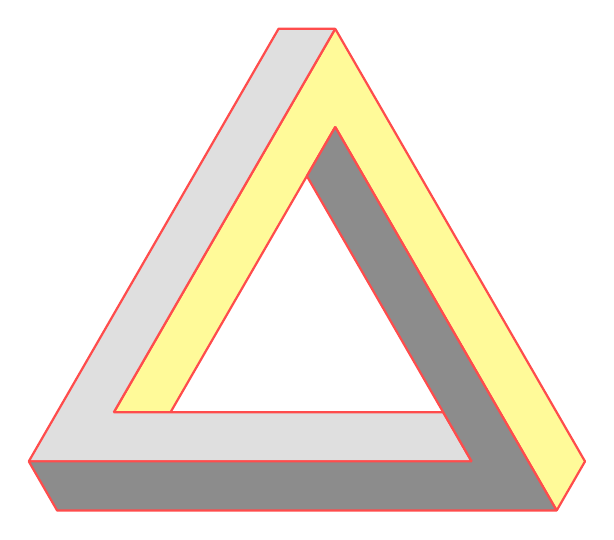
\begin{tikzpicture}[scale=0.8, line join=bevel]
    \pgfmathsetmacro{\a}{2.5}
    \pgfmathsetmacro{\b}{0.9}

    \tikzset{%
      apply style/.code     = {\tikzset{#1}},
      triangle_edges/.style = {thick,draw=red!70}
    }
    \foreach \theta/\facestyle in {%
        0/{triangle_edges, fill = yellow!40},
      120/{triangle_edges, fill = gray!25},
      240/{triangle_edges, fill = gray!90}%
    }{
      \begin{scope}[rotate=\theta]
        \draw[apply style/.expand once=\facestyle]
          ({-sqrt(3)/2*\a},{-0.5*\a})                     --
          ++(-\b,0)                                       --
            ({0.5*\b},{\a+3*sqrt(3)/2*\b})                -- % higher point	
            ({sqrt(3)/2*\a+2.5*\b},{-.5*\a-sqrt(3)/2*\b}) -- % rightmost point
          ++({-.5*\b},-{sqrt(3)/2*\b})                    -- % lower point
            ({0.5*\b},{\a+sqrt(3)/2*\b})                  --
          cycle;
        \end{scope}
      }	
\end{tikzpicture}
\end{center}







\newpage

\section{简明数理逻辑}

数理逻辑是研究推理规则的数学分支。
而本章仅仅介绍数理逻辑的一些主要概念、基本原理,不打算进一步深究。
在本章,我们常用的自然语言(中文 or English)中的表达逻辑关系、推理证明的各个要素
将会被逐步地符号化,即通过构造各种符号语言来代替自然语言,
最终得到完全由符号构成的形式语言。为达到这个邪恶的目的,
在本章第一节我们首先将关联词语(逻辑连接词)符号化,比如:
不但而且、虽然但是、因为所以、如果那么、只要就、只有才……等等……

\subsection{命题与连接词}
\textbf{命题}数理逻辑中的一个基本概念。
能够判断真假,非真即假的陈述句称为命题。

\begin{example}下列语句之中,(1)-(3)都是命题,而(4)-(6)不是命题:

(1)加拿大位于北美洲;

(2)$1+1=3$;

(3)公元2333年元旦的北京是晴天;

(4)你脑子进屎了吗?

(5)让我们荡起双桨;

(6)这句话是假话。\label{examples of propositions}
\end{example}

(1)(2)(3)都是可以判断真假的陈述句,
从而是命题,虽然(2)陈述的事实是荒谬的。
而对于(3),我们目前没有能力判断它到底是真还是假,
但它的真假性是客观存在的,这样的语句也是命题。

(4)(5)都不是陈述句,从而不是命题。
而(6)虽然是陈述句,但它的真假不确定,
假设它为真则推出它为假,由它为假又能推出它为真。
这种既不能为真也不能为假的陈述句,称为\textbf{悖论}。悖论不是命题。\vsp

我们用小写拉丁字母,如$a,b,c,p,q,r$等,来表示命题。
如果一个命题为真,则称它为\textbf{真命题},也称它的\textbf{真值}为1;若它为假,
则称此命题为\textbf{假命题},也称它的真值为0.\vsp

对于已经给定的一些命题,我们可以对这些命题进行一些操作,
来构造新的命题。接下来介绍常见的几种命题连接词。

\begin{definition}[否定连接词]
对于命题$p$,称命题$\neg p$为$p$的\textbf{否定式},
符号“$\neg$”称为否定连接词,读作“\textbf{非}”。
规定当$p$为真时,$\neg p$为假;$p$为假时$\neg p$为真。
\end{definition}
在自然语言中,命题“$\neg p$”可以表达为“$p$不成立”。
例如命题$p$表示“加拿大位于北美洲”,则$\neg p$表示“加拿大不位于北美洲”。

\begin{definition}[合取连接词]
对于两个命题$p,q$,称命题“$p\wedge q$”为$p$与$q$的\textbf{合取式},
符号“$\wedge$”称为合取连接词,读作“\textbf{且}”。
规定当$p,q$全都是为真命题时,$p\wedge q$为真命题;
当$p,q$之中至少有一个是假命题时,$p\wedge q$为假命题。
\end{definition}
对于两个命题$p,q$,$p\wedge q$用自然语言可以描述为
“$p$与$q$同时成立”、“$p$与$q$全都正确”、“$p$并且$q$”、
“虽然$p$但是$q$”、“不仅$p$而且$q$”、“both $p$ and $q$ are true”等等。

特别注意自然语言中的“但是”和“并且”,
其实表达的都是$\wedge$的意思,指两者同时成立。

\begin{definition}[析取连接词]
对于两个命题$p,q$,称命题“$p\vee q$”为$p$与$q$的\textbf{析取式},
符号“$\vee$”称为析取连接词,读作“\textbf{或}”。
规定当$p,q$全都是为假命题时,$p\vee q$为假命题;
当$p,q$之中至少有一个是真命题时,$p\vee q$为真命题。
\end{definition}
对于两个命题$p,q$,“$p\vee q$”在自然语言中常称为“$p$或者$q$”.
然而特别注意,“或者”这个词在汉语中有歧义,
在有些语境下表示“两者当中有且只有一个成立”,
例如“你滚蛋,或者我滚蛋”。但是在数理逻辑中,
“或者”指的是两者至少有一个成立就可以(两者都成立那更好)。

\begin{definition}[蕴含连接词]
对于两个命题$p,q$,称命题“$p\rightarrow q$”为$p$与$q$的\textbf{蕴含式},
符号“$\rightarrow$”称为蕴含连接词,读作“\textbf{蕴含}”。
规定当$p$为真命题并且$q$为假命题时,$p\rightarrow q$为假命题;
而其余3种情况时$p\rightarrow q$为真命题。
\end{definition}

对于两个命题$p,q$,“$p\rightarrow q$”在自然语言和今后我们要学习的数学当中,有
“如果$p$那么$q$”,“$p$仅当$q$”,“$p$推出$q$”,
“因为$p$所以$q$”,“只要$p$就有$q$”,“只有$q$才会有$p$”,“除非$q$否则$p$”、
“$p$是$q$的\textbf{充分条件}”,“$q$是$p$的\textbf{必要条件}”等
看似迥异的表述方式。

上述诸多表达方式在数理逻辑中其实表达的都是“蕴含”的含义,这需要慢慢体会。

蕴含连接词也许是在本节所讲的所有连接词中最令初学者费解的一个。
为帮助读者理解,我们举一些例子来说明:

\begin{example}研究下列命题。
虽然它们表达的含义荒诞至极,但在数理逻辑的意义下它们都是真命题:

(1)因为所有人都吃过屎,所以地球围绕太阳公转。

(2)如果1+1=3,那么猪会飞。

(3)只有沙漠能下暴雨,大海才会亲吻鲨鱼。

(4)只要2是奇数,公元2333年元旦的北京就是晴天。
\end{example}
\begin{proof}
我们依次来分析这些命题:

(1)我们用字母$p$来表示“所有人都吃过屎”,用$q$来表示“地球围绕太阳公转”。
则命题(1)用符号表达为“$p\rightarrow q$”.由于$p$是假命题,$q$是真命题,
所以根据蕴含连接词"$\rightarrow$"的定义可知$p\rightarrow q$为真命题。

(2)该命题为“$(1+1=3)\rightarrow\text{猪会飞}$”。
由于“1+1=3”是假命题,“猪会飞”也是假命题,从而命题(2)是真命题。

(3)该命题为“大海亲吻鲨鱼$\rightarrow$沙漠下暴雨”,
蕴含连接词的前后两端都是假命题,从而这个命题是真命题。

(4)该命题为“2是奇数$\rightarrow$公元2333年元旦的北京是晴天”。
我们知道“2是奇数”是假命题。虽然我们并没有能力判断公元2333年那件事的真假,
但是从蕴含连接词的定义可以看出,
对于一个由蕴含连接词连接的复合命题$p\rightarrow q$,只要$p$是假命题,
那么无论$q$是真是假,$p\rightarrow q$一定是真命题。从而命题(4)是真命题。
\end{proof}

要特别注意,在日常生活的自然语言中,
“如果$p$那么$q$”中的$p,q$之间通常有内在的联系,
因果联系、依赖关系等等。
而数理逻辑研究的是抽象的推理,
“命题”本身是一个剥离于现实世界的抽象的概念,
我们谈论命题“$p\rightarrow q$”时,$p$与$q$之间可以毫无任何联系。
命题“$p\rightarrow q$”的真假性,只与$p,q$两者的真假性有关,
而与它们所表达的实际意义之间有何内在联系无关。
这对于其它几个逻辑连接词,也都是如此。

我们再看一些关于蕴含连接词的例子:

\begin{example}
甲、乙两个人比赛,甲对此信心满满,说:“如果我输了,我给你100块钱。”
试将命题“如果甲输,那么甲给乙100块钱”符号化,并讨论该命题何时为假命题。
\end{example}
\begin{proof}[Solution]
此命题为“甲输$\rightarrow$甲给乙100块钱”。
只有当甲输了但是甲没给乙100块钱时,
甲所讲的这个命题才是假的。特别注意当甲赢了时候(即“甲输”为假命题),
无论甲有没有给钱,那句话都是真命题。
\end{proof}

这个实际例子也许能够帮助初学者理解为很么要规定当前提$p$为假命题时
$p\rightarrow q$ 一定是真命题。事实上,再以后的学习中,我们会接触到更多
抽象的结构(比如拓扑空间、概率空间等),
它们的严格定义会令初学者费解。之所以要如此定义,
是因为这样定义出来的东西具有我们所希望的性质——这正是近代数学的特色之一。
我们在下一节会介绍“所希望的性质”具体是什么(见下一节的定理\ref{prop-dengzhi-gongshi-3})。

\begin{example}假设你是人(这是确凿无疑的),试判断下列命题的真假:

(1)如果你是人,那么你不是人。

(2)如果你不是人,那么你是人。

(3)你是人,并且你不是人。

(4)除非你是人,否则你不是人。
\end{example}

\begin{proof}[Solution]
我们用字母$p$表示命题“你是人”,则$p$为真命题(希望读者承认这个事实)。
则上述4个命题用符号来表达,分别为
$$p\rightarrow (\neg p)\,\,\,,\,\,\,
(\neg p)\rightarrow p\,\,\,,\,\,\,
p\wedge(\neg p)\,\,\,,\,\,\,
(\neg p)\rightarrow p$$
由相应连接词的运算规则,不难得出(1)(3)为假命题,(2)(4)为真命题。
\end{proof}

\begin{definition}[等价连接词]
对于两个命题$p,q$,称命题“$p\leftrightarrow q$”为$p$与$q$的\textbf{等价式},
符号“$\leftrightarrow$”称为等价连接词,读作“\textbf{等价于}”。
规定当$p,q$真值相同时$p\leftrightarrow q$为真命题;
真值相反时$p\leftrightarrow q$为假命题。
\end{definition}
在自然语言以及数学中,常用“$p$\textbf{当且仅当}$q$”、“$p$是$q$的\textbf{充要条件}”、
“$p$ \textbf{if and only if} $q$”来表达命题“$p\leftrightarrow q$”.\vsp

以上是常见的五种逻辑连接词。
我们将由连接词组成的复合命题的真假性总结为如下\textbf{真值表}:

$$\begin{tabular}{|c||c|c|c|c|c|}   % |:竖线, l、c、r := 居左,居中,居右
\hline
$p\,\,q$ & $\neg p$ & $p\wedge q$ & $p\vee q$ & $p\rightarrow q$ & $p\leftrightarrow q$\\
\hline
$0\,\,0$ & 1 & 0 &0&1&1 \\

$0\,\,1$ & 1 & 0 &1&1&0 \\

$1\,\,0$ & 0 & 0 &1&0&0 \\

$1\,\,1$ & 0 & 1 &1&1&1 \\
\hline
\end{tabular}$$

例如,从表中第一行可以看出,当$p,q$都是假命题(真值为0)时,
$\neg p$、$p\wedge q$、$p\vee q$、$p\rightarrow q$、$p\leftrightarrow q$的真值
分别为1、0、0、1、1.\vsp

由简单的命题,以及各种逻辑连接词,可以构造出复杂的命题。
例如对于命题$p,q,r,s$,我们可以去谈论诸如
$$((\neg p)\vee r)\wedge(s\leftrightarrow q)$$
这样的复杂命题。这种命题的真假性完全由$p,q,r,s$之中每一个命题的真假性决定。\vs

在本节最后,我们再简单提一下逻辑连接词运算的\textbf{优先级}。
与实数加减乘除运算规则“先乘除后加减,有括号先算括号里面的”类似,
我们也约定各种逻辑连接词的优先级。规定优先顺序为
$$\neg\,>\,\wedge\,>\,\vee\,>\,\rightarrow\,>\,\leftrightarrow$$

例如,命题$\neg p\vee q$确切地说应该是$(\neg p)\vee q$,而不是$\neg(p\vee q)$.
再比如,命题$p\vee q\leftrightarrow r\wedge s$所表达的含义是
$(p\vee q)\leftrightarrow (r\wedge s)$,而不是$((p\vee q)\leftrightarrow r)\wedge s$.

在以后,我们尽量避免依靠这个优先级约定规则,而是尽可能多加括号减少歧义。


\subsection{命题逻辑等值演算(待补)}
在初等数学中我们用字母(比如$x$)表示实数。
在一些语境下,$x$是一个确定的数,
而在有些语境下字母$x$代表的数不确定——
这正是\textbf{常量}与\textbf{变量}的区别。
比如“$x^2+1$”,在某些语境下,$x$是一个确定的数,
那$x^2+1$就是一个确定的数;而在另一些语境下,
$x^2+1$是一个公式,我们给$x$赋以特定的值,就会得到$x^2+1$的一个值。
特别注意一个字母到底代表常量还是变量,
需要依靠事先约定以及语境来判断。\vs

而命题逻辑与之完全类似。我们用字母来表示一个命题。
命题也有\textbf{命题常量}与\textbf{命题变量}之分。
前者为某个确定的命题,而后者是一个抽象的符号,
可以被赋以确定的命题。

\begin{definition}[命题公式]
由命题常量、命题变量、逻辑连接词、括号$()$按照某些逻辑关系
所排列而成的符号串称为命题公式。具体地,“某些逻辑关系”指的是:

(1)对于单个命题常量或者命题变量$p$,
由符号$p$自身构成的符号串是命题公式。

(2)如果符号串$A,B$都是命题公式,那么符号串
$$(\neg A)$$
$$(A\vee B)$$
$$(A\wedge B)$$
$$(A\rightarrow B)$$
$$(A\leftrightarrow B)$$
都是命题公式。
\end{definition}

注意“命题公式”这个概念是\textbf{归纳定义}
(或者叫\textbf{递归定义})的。
通俗地说,命题公式是由有限多个命题常量、有限多个命题变量,
经过命题连接词的有限多步连接,所构成的符号串。

例如,我们用字母$p$来表示命题“地球绕太阳公转”,那么符号串
$$((\neg p)\vee q)\leftrightarrow(r\rightarrow p)$$
是一个命题公式。其中$q,r$是命题变量,而$p$是命题常量。
这个命题公式含有2个命题变量。特别注意,命题公式可以不含有命题变量。

再注意一点,命题连接词除了我们提到的5种(否定、合取、析取、蕴含、等价)之外,
还有无数多种;只不过这5种比较“常用”,自然语言中存在表达其含义的词汇。
而其它一些连接词,它表达的逻辑关系是“无法言说的”(无法用正常的“人话”轻易讲清楚),
自然语言在其面前苍白无力。我们在本章习题中会提到一些其它的连接词。
事实上,在习题中我们还将证明“$\neg,\vee$”这两个连接词在某种意义下已经“足够用”了。

对于用这5种连接词之外的连接词来连接的字符串,
我们也认为是命题公式。这在本章习题中会略加讨论。

\begin{definition}[命题公式的赋值]
设字符串$A=A(p_1,...,p_n)$是含有$n$个命题变量$p_1,p_2,...,p_n$的
一个命题公式。对每个$p_1,...,p_n$各指定一个真值,
称为命题公式$A$的一个\textbf{赋值}(或者称为“\textbf{诠释}”)。
\end{definition}

容易知道,对于含有$n$个命题变量的命题公式$A$,
$A$总共有$2^n$种不同的赋值。(这是因为对于每个命题变量,
要么赋以它真值0,要么赋以它真值1,一共2种选择;而共有$n$个变量,从而总共
$2\times 2\times...\times2=2^n$种赋值)

回顾上一节出现的\textbf{真值表}。对于命题公式,
我们可以穷尽它所有可能的赋值,并把每一种赋值及其结果一一列出。

\begin{example}我们考虑关于命题变量$p,q,r$的下述三个命题公式
$$A:=p\rightarrow (q\rightarrow r)$$
$$B:=(p\wedge q)\rightarrow r$$
$$C:=(p\rightarrow q)\rightarrow r$$
试讨论它们所有可能的赋值,并总结为真值表。
\label{proposition formula}
\end{example}
\begin{proof}[Solution]
逐一讨论所有可能的$2^3=8$种赋值,总结为下表:

$$\begin{tabular}{|c||c|c|c|}   % |:竖线, l、c、r := 居左,居中,居右
\hline
$p\,\,q\,\,r$ & $p\rightarrow (q\rightarrow r)$
& $(p\wedge q)\rightarrow r$ & $(p\rightarrow q)\rightarrow r$ \\
\hline
$0\,\,0\,\,0$ & 1 & 1 & 0  \\
$0\,\,0\,\,1$ & 1 & 1 & 1  \\
$0\,\,1\,\,0$ & 1 & 1 & 0  \\
$0\,\,1\,\,1$ & 1 & 1 & 1  \\
$1\,\,0\,\,0$ & 1 & 1 & 1  \\
$1\,\,0\,\,1$ & 1 & 1 & 1  \\
$1\,\,1\,\,0$ & 0 & 0 & 0  \\
$1\,\,1\,\,1$ & 1 & 1 & 1  \\
\hline
\end{tabular}$$
按照相应逻辑连接词的运算规则,读者可自行验证上述结果。
\end{proof}

注意观察上述真值表的(从双竖线右边起)第1、2列,发现它们完全相同。
也就是说,对于公式
$p\rightarrow (q\rightarrow r)$与$(p\wedge q)\rightarrow r$,
无论对变量$p,q,r$赋予哪些真值,所得到的命题的真值都相同。

与初等数学类比一下,这就好比含有变量$x,y$的两个表达式
$$2(x+2y)\,\,\,\,,\,\,\,\,2x+4y$$
无论对$x,y$赋予什么值,所得到的结果都相等。
(但实数有无限多个,我们无法一一列出上述式子所有可能的赋值,
总结成类似的真值表。
所以在这种意义下,命题逻辑比初等代数简单得多。)\vs

在初等数学中,我们并不是通过暴力验证对变量$x,y$的每一种可能的赋值,
来证明$2(x+2y)$与$2x+4y$是“相等”的(事实上暴力穷举是不现实的,毕竟实数有无限多个),
而是通过一些\textbf{运算律};而命题逻辑的简单之处在于
我们可以暴力地验证所有可能的赋值来说明两个命题公式其实是“相等”的。
事实上暴力验证可以交给计算机来完成。

\begin{definition}[命题公式的分类]
对于含有$n$个$(n\geq0)$命题变量的命题公式$A=A(p_1,...,p_n)$,

(1)称$A$为\textbf{重言式}(或者\textbf{永真式}),
如果在$A$的任何赋值下,$A$的结果都为真;

(2)称$A$为\textbf{矛盾式}(或者\textbf{永假式}),
如果在$A$的任何赋值下,$A$的结果都为假;

(2)称$A$为\textbf{可满足式},
如果存在$A$的某个赋值,使得$A$的结果为真;
\end{definition}

从定义容易看出,重言式一定是可满足式。

顺便提一下$n=0$这种\textbf{平凡}(trivial)的情形,即$A$为含有0个命题变量的命题公式的情形。
此时$A$无非就是一个命题常量。
$A$为重言式当且仅当$A$为真命题当且仅当$A$为可满足式;
$A$为矛盾式当且仅当$A$为假命题。\vs

判断一个命题公式是否为重言式、可满足式、矛盾式,
我们可以用真值表的方法。
即,穷尽所有可能的赋值。例如,在刚才的例子\ref{proposition formula}
之中出现的三个命题公式都是可满足式,都不是重言式——从它们的真值表中能轻易看出来。

\begin{definition}[命题公式的等值]
对于含有$n$个命题变量$p_1,...,p_n$的两个命题公式$A,B$,
称$A$与$B$\textbf{等值},如果在所有可能的$2^n$个赋值之下,它们的真值都相同。
此时记作$A\Leftrightarrow B$.
\end{definition}
例如,例子\ref{proposition formula}之中的两个命题公式$A,B$是等值的,
这从真值表中可以看出来。
用符号语言表示为
$$[p\rightarrow (q\rightarrow r)]
\Leftrightarrow [(p\wedge q)\rightarrow r]$$
特别需要注意的是,符号“$\Leftrightarrow$”并不是逻辑连接词,
不要与$\leftrightarrow$混淆。不过它们两者之间有如下联系:

\begin{thm}对于含有$n$个命题变量$p_1,...,p_n$的命题公式$A,B$,则
$A\Leftrightarrow B$当且仅当$A\leftrightarrow B$是重言式。
\end{thm}
\begin{proof}
这根据“等值$\Leftrightarrow$”、“重言式”、“命题连接词$\leftrightarrow$”的定义,
直接得到。几乎是显然的。不过在此还是要详细写一下证明,给初学者。

一方面在$A\Leftrightarrow B$的条件下,我们将证明$A\leftrightarrow B$是重言式。
根据重言式的定义,我们只需要证明,对于变量$p_1,...,p_n$的任何赋值,得到的命题
$A(p_1,...,p_n)\leftrightarrow B(p_1,...,p_n)$是真命题。
而这是因为,由于$A\Leftrightarrow B$,从而
$A(p_1,...,p_n)$与$B(p_1,...,p_n)$的真值总是相同,因此由逻辑连接词$\leftrightarrow$
的运算规则知$A(p_1,...,p_n)\leftrightarrow B(p_1,...,p_n)$是真命题,
这对任何赋值都成立。从而$A\leftrightarrow B$是重言式。

另一方面,我们还要证明在$A\leftrightarrow B$是重言式的条件下,
有$A\Leftrightarrow B$.方法完全类似(刚才的证明过程处处可逆),读者自行完成。
\end{proof}

接下来将介绍一些常见的命题公式等值式。

\begin{thm}[基本的命题公式等值式I]\label{prop-dingzhi-gongshi-1}
设$A$为任意的命题公式,则下列成立:

(1)零律:$$A\vee1\Leftrightarrow1$$
$$A\wedge0\Leftrightarrow0$$

(2)同一律:$$A\wedge1\Leftrightarrow A$$
$$A\vee0\Leftrightarrow A$$

(3)幂等律:$$A\Leftrightarrow A\vee A$$
$$A\Leftrightarrow A\wedge A$$

(4)双重否定律:$$A\Leftrightarrow \neg(\neg A)$$

(5)排中律:$$A\vee\neg A\Leftrightarrow1$$

(6)矛盾律:$$A\wedge\neg A\Leftrightarrow0$$

\end{thm}
\begin{proof}
这些都是显然的,直接用真值表验证即可(考虑$A$的真值为$0,1$的两种情况即可)。
\end{proof}

特别注意,上述等值式中的$A$可以被替换为任何命题公式。
比如令$A$为含有3个命题变量的命题公式$(p\rightarrow q)\rightarrow r$,则
幂等律(3)变为
$$(p\rightarrow q)\rightarrow r
\Leftrightarrow [(p\rightarrow q)\rightarrow r]\vee [(p\rightarrow q)\rightarrow r]$$
$$(p\rightarrow q)\rightarrow r
\Leftrightarrow [(p\rightarrow q)\rightarrow r]\wedge [(p\rightarrow q)\rightarrow r]$$
这仍然是命题等值式。上述$p,q,r$也可以继续被替换为更复杂的命题公式。

\begin{thm}[基本的命题公式等值式II]\label{prop-dengzhi-gongshi-2}
对于任何命题公式$A,B,C$,则下列等值式成立:

(7)交换律:$$A\wedge B\Leftrightarrow B\wedge A$$
$$A\vee B\Leftrightarrow B\vee A$$

(8)结合律:$$(A\wedge B)\wedge C\Leftrightarrow A\wedge (B\wedge C)$$
$$(A\vee B)\vee C\Leftrightarrow A\vee (B\vee C)$$

(9)分配律:
$$(A\wedge B)\vee C\Leftrightarrow (A\vee C)\wedge (B\vee C)$$
$$(A\vee B)\wedge C\Leftrightarrow (A\wedge C)\vee (B\wedge C)$$

(10)吸收律:
$$A\vee (A\wedge B)\Leftrightarrow A$$
$$A\wedge (A\vee B)\Leftrightarrow A$$

(11)德摩根律:
$$\neg(A\vee B)\Leftrightarrow\neg A\wedge\neg B$$
$$\neg(A\wedge B)\Leftrightarrow\neg A\vee\neg B$$

\end{thm}

\begin{proof}
对命题公式$A,B,C$被赋值之后所得到的命题的真假进行讨论,
用真值表暴力验证即可。

我们先来看交换律(7).列出真值表,见下表:
$$\begin{tabular}{|c||cc|cc|}   % |:竖线, l、c、r := 居左,居中,居右
\hline
$A\,\,B$ & $A\wedge B$ & $B\wedge A$ & $A\vee B$ & $B\vee A$\\
\hline
$0\,\,0$ & 0 & 0 & 0 & 0  \\
$0\,\,1$ & 0 & 0 & 1 & 1  \\
$1\,\,0$ & 0 & 0 & 1 & 1  \\
$1\,\,1$ & 1 & 1 & 1 & 1  \\
\hline
\end{tabular}$$
观察此真值表各列,容易发现相应的等值关系。

接下来看(8)结合律,我们暴力列出如下真值表:

$$\begin{tabular}{|c||cc|cc|}   % |:竖线, l、c、r := 居左,居中,居右
\hline
$A\,\,B\,\,C$ & $(A\wedge B)\wedge C$ & $A\wedge (B\wedge C)$
& $(A\vee B)\vee C$ & $A\vee (B\vee C)$\\
\hline
$0\,\,0\,\,0$ & 0 & 0 & 0 & 0  \\
$0\,\,0\,\,1$ & 0 & 0 & 1 & 1  \\
$0\,\,1\,\,0$ & 0 & 0 & 1 & 1  \\
$0\,\,1\,\,1$ & 0 & 0 & 1 & 1  \\
$1\,\,0\,\,0$ & 0 & 0 & 1 & 1  \\
$1\,\,0\,\,1$ & 0 & 0 & 1 & 1  \\
$1\,\,1\,\,0$ & 0 & 0 & 1 & 1  \\
$1\,\,1\,\,1$ & 1 & 1 & 1 & 1  \\
\hline
\end{tabular}$$
分配律、吸收律、德摩根律的证明完全类似,留给读者完成。
\end{proof}

关于等价、蕴含连接词,还有如下等值式:

\begin{thm}[基本的命题公式等值式III]\label{prop-dengzhi-gongshi-3}
设$A,B$为任意的命题公式,则成立下列命题公式等值式:

(12)蕴含律:
$$A\rightarrow B\Leftrightarrow\neg A\vee B$$

(13)等价律:
$$A\leftrightarrow B\Leftrightarrow (A\rightarrow B)\vee(B\rightarrow A)$$

(14)假言易位:
$$A\rightarrow B\Leftrightarrow\neg B\rightarrow\neg A$$

(15)等价否定:
$$A\leftrightarrow B\Leftrightarrow\neg A\leftrightarrow\neg B$$

(16)归谬论:
$$(A\rightarrow B)\wedge(A\rightarrow\neg B)\Leftrightarrow\neg A$$
\end{thm}
\begin{proof}
用真值表的方法暴力验证蕴含律和等价律,读者自行完成,在此从略。
假言易位、等价否定、归谬论也可以用真值表,但其实我们不必那么暴力,
因为这三者可以由之前所证明过的等值式推出来。

对于任意两个命题公式$A,B$,有
$$\begin{tabular}{cll}   % |:竖线, l、c、r := 居左,居中,居右
&$A\rightarrow B$&\\
$\Leftrightarrow$& $\neg A\vee B$ &\text{(蕴含律)}\\
$\Leftrightarrow$& $B\vee \neg A$ &\text{(交换律)}\\
$\Leftrightarrow$& $\neg(\neg B)\vee\neg A$ &\text{(双重否定律)}\\
$\Leftrightarrow$& $\neg B\rightarrow\neg A$ &\text{(蕴含律)}\\
\end{tabular}$$
从而假言易位(14)得证。

再注意到
$$\begin{tabular}{cll}   % |:竖线, l、c、r := 居左,居中,居右
&$A\leftrightarrow B$&\\
$\Leftrightarrow$& $(A\rightarrow B)\wedge(B\rightarrow A)$ &\text{(等价律)}\\
$\Leftrightarrow$& $(\neg B\rightarrow\neg A)\wedge(\neg A\rightarrow \neg B)$ &\text{(假言易位)}\\
$\Leftrightarrow$& $(\neg A\rightarrow \neg B)\wedge(\neg B\rightarrow\neg A)$ &\text{(交换律)}\\
$\Leftrightarrow$& $\neg A\leftrightarrow\neg B$ &\text{(等价律)}\\
\end{tabular}$$
从而等价否定(15)得证。

最后注意到
$$\begin{tabular}{cll}   % |:竖线, l、c、r := 居左,居中,居右
&$(A\rightarrow B)\wedge(A\rightarrow \neg B)$&\\
$\Leftrightarrow$&
$(\neg A\vee B)\wedge(\neg A\vee\neg B)$ &\text{(蕴含律)}\\
$\Leftrightarrow$&
$[\neg A\wedge(\neg A\vee\neg B)]\vee
[B\wedge(\neg A\vee\neg B)]$ &\text{(分配律)}\\
$\Leftrightarrow$&
$(\neg A)\vee
[B\wedge(\neg A\vee\neg B)]$ &\text{(吸收律)}\\
$\Leftrightarrow$&
$(\neg A)\vee
[(B\wedge\neg A)\vee(B\wedge\neg B)]$ &\text{(交换律,分配律)}\\
$\Leftrightarrow$&
$[(\neg A)\vee
(B\wedge\neg A)]\vee0$ &\text{(结合律,矛盾律)}\\
$\Leftrightarrow$&
$(\neg A)\vee
(\neg A\wedge B)$ &\text{(同一律,交换律)}\\
$\Leftrightarrow$&
$\neg A$ &\text{(吸收律)}\\
\end{tabular}$$
从而归谬论(16)得证。
\end{proof}

像这样来通过已知的等值式(运算律)
来得到新的等值式的方式被称为\textbf{等值演算}。

其实,在上述等值演算的过程中,我们“偷偷地”使用了以下重要规则:

\begin{thm}[置换规则]
设$\Phi(A)$是含有命题公式$A$的命题公式,$B$是另一个命题公式。
如果$A\Leftrightarrow B$,那么必有$\Phi(A)\Leftrightarrow\Phi(B)$.
\end{thm}
这个道理几乎是显然的,由等值“$\Leftrightarrow$”的定义容易得到。
我们在定理\ref{prop-dengzhi-gongshi-3}的(14)-(16)
的证明过程中已经使用了置换规则。此规则是等值演算的基础。
另外一个显然的事实也十分重要:

\begin{thm}[等值关系是等价关系]对于任意的命题公式$A,B,C$,下列成立

(1)(自反性)$A\Leftrightarrow A$.

(2)(对称性)如果$A\Leftrightarrow B$,那么$B\Leftrightarrow A$.

(3)(传递性)如果$A\Leftrightarrow B$并且$B\Leftrightarrow C$,
那么$A\Leftrightarrow C$.
\end{thm}

这个也容易证明,几乎是显然的。\vsp

接下来我们举一些等值演算的例子,来结束本节。

\begin{example}
我们重新来看例子\ref{proposition formula}之中出现的
关于$3$个命题变量$p,q,r$的命题公式。我们已经用真值表的方法知道了
$$p\rightarrow (q\rightarrow r)\Leftrightarrow
(p\wedge q)\rightarrow r$$
现在,用等值演算的方法再次得到此等值式。
\end{example}
\begin{proof}[Solution]
运用我们所介绍的基本的运算律,容易知道
$$\begin{tabular}{cll}
&$p\rightarrow (q\rightarrow r)$&\\
$\Leftrightarrow$& $p\rightarrow (\neg q\vee r)$ & \text{(蕴含律)}\\
$\Leftrightarrow$& $\neg p\vee (\neg q\vee r)$ & \text{(蕴含律)}\\
$\Leftrightarrow$& $(\neg p\vee\neg q)\vee r$ & \text{(结合律)}\\
$\Leftrightarrow$& $\neg(p\wedge q)\vee r$ & \text{(德摩根律)}\\
$\Leftrightarrow$& $(p\wedge q)\rightarrow r$ & \text{(蕴含律)}\\
\end{tabular}$$
从而得证,比暴力计算真值表要方便。
\end{proof}

建议初学者学习等值演算时,像本节一样,每一步演算都标注上所使用的运算律。
等到熟练时,就不必在每一步的右边添加括号备注了。

\begin{example}[又一个常用的关于等价的等值关系]
对于命题变量$p,q$,证明等值式
$$p\leftrightarrow q\Leftrightarrow
(p\wedge q)\vee(\neg p\wedge\neg q)$$\label{dengjialv-ii}
\end{example}
\begin{proof}
只需注意到
$$\begin{tabular}{cll}
&$p\leftrightarrow q$&\\
$\Leftrightarrow$&$(p\rightarrow q)\wedge(q\rightarrow p)$
&\text{(等价律)}\\
$\Leftrightarrow$&$(\neg p\vee q)\wedge(\neg q\vee p)$
&\text{(蕴含律)}\\
$\Leftrightarrow$&$(\neg p\wedge\neg q)\vee(\neg p\wedge p)
\vee(q\wedge\neg q)\vee(q\wedge p)$
&\text{(反复使用分配律)}\\
$\Leftrightarrow$&$(\neg p\wedge\neg q)\vee0
\vee0\vee(q\wedge p)$
&\text{(矛盾律)}\\
$\Leftrightarrow$&$(\neg p\wedge\neg q)\vee(q\wedge p)$
&\text{(同一律)}\\
$\Leftrightarrow$&$(p\wedge q)\vee(\neg p\wedge\neg q)$
&\text{(交换律)}\\
\end{tabular}$$
从而证毕。
\end{proof}

事实上,用自然语言去想,这个结果是显然的。
$p\leftrightarrow q$的意思是“$p$与$q$等价”;而
$(p\wedge q)\vee(\neg p\wedge\neg q)$翻译成自然语言为
“$p$与$q$同时成立或者同时不成立”。从而可知它们表达同一个含义。

\begin{example}考虑含有$p,q,r$三个命题变量的命题公式
$$(p\leftrightarrow(\neg q\vee r))\rightarrow
(\neg p\rightarrow q)$$
判断它是否为重言式。
\end{example}
\begin{proof}[Solution]我们介绍三种方法。

方法一:鉴于一共只含3个命题变量,我们完全可以用真值表法来判断,
讨论所有可能的$2^3=8$种赋值即可。容易知道它是重言式。\vs

方法二:等值演算法。其实这也是一种暴力的方法,用它总能做出来。
演算的原则是先利用蕴含律、等价律,把$\leftrightarrow,\rightarrow$
完全用$\wedge,\vee,\neg$表示出来,得到只含有$\wedge,\vee,\neg$
这三个连接词的命题公式;再之后反复使用交换律、结合律、分配律、吸收律、摩根律
(也就是定理\ref{prop-dengzhi-gongshi-2}“第II组等值式”之中的);最后用“第I组”等值式。
本例的具体过程如下:
$$\begin{tabular}{cll}
&$(p\leftrightarrow(\neg q\vee r))\rightarrow
(\neg p\rightarrow q)$&\\

$\Leftrightarrow$&
$[(p\wedge(\neg q\vee r))\vee(\neg p\wedge\neg(\neg q\vee r))]\rightarrow
(\neg p\rightarrow q)$
&\text{(用例子\ref{dengjialv-ii}杀掉等价连接词)}\\

$\Leftrightarrow$&
$\neg[(p\wedge(\neg q\vee r))\vee(\neg p\wedge\neg(\neg q\vee r))]\vee
(p\vee q)$
&\text{(用蕴含律杀掉蕴含连接词)}\\

$\Leftrightarrow$&
$[(\neg p\vee(q\wedge\neg r))\wedge(p\vee\neg q\vee r))]\vee
(p\vee q)$
&\text{(反复使用德摩根律、双重否定律)}\\

$\Leftrightarrow$&
$[\neg p\vee(q\wedge\neg r)\vee(p\vee q)]
\wedge[p\vee(\neg q\vee r)\vee(p\vee q)]$
&\text{(分配律)}\\

$\Leftrightarrow$&
$[(\neg p\vee p)\vee(q\wedge\neg r)\vee q]
\wedge[(\neg q\vee q)\vee p\vee r\vee p]$
&\text{(交换律、结合律)}\\

$\Leftrightarrow$&
$[1\vee(q\wedge\neg r)\vee q]
\wedge[1\vee p\vee r\vee p]$
&\text{(排中律)}\\

$\Leftrightarrow$&
$1\wedge1$
&\text{(零律)}\\

$\Leftrightarrow$&$1$&\text{(连接词$\wedge$的定义)}\\
\end{tabular}$$
从而原命题公式与真命题$1$是等值的,说明原命题公式是重言式。
\end{proof}

\subsection{推理与证明(待补)}
\subsection{主体与谓词逻辑(待补)}
\subsection{量词与一阶逻辑(待补)}
\subsection{一阶逻辑等值演算与推理(待补)}
\subsection{数学归纳法(待补)}
\subsection{习题(待补)}

\section{朴素集合论}
\subsection{集合的概念与基本例子}
\begin{definition}
集合的概念不可言说,不言自明,无须定义。谓词$\in$(读作“属于”)也不可言说。两个集合的相等,也无需定义。
\end{definition}
粗俗地说,“几乎所有你能想到的”的事物、对象,都是集合。
而两个集合相等,通俗地说就是它们是同一个事物。
对于两个集合$A,B$,我们可以构造出命题$A\in B$.当$A\in B$为真命题时,我们称
$A$是$B$的元素。

为避免集合论悖论,我们简单粗暴地避开谈论$A\in A$这个命题。我们不认为一个集合是它自身的元素。
例如,所有集合构成的全体,我们不认为是集合。事实上,并不是随便一些东西放在一起都构成一个集合。
哪些东西放在一起构成集合,哪些不认为是集合,是被集合论公理体系规定的,本讲义不打算深究。
本章最末会对集合论公理做简单介绍。\vs

由所有满足性质$P$的对象$x$的全体构成的集合,记作
$$\{x|P(x)\}$$

当然,对于某些集合,我们也可以通过列举其中的元素来表示这个集合,例如由$1,2,3$
这三个元素构成的集合可以记为$\{1,2,3\}$.

关于集合相等,首先有一条基本的公理:\vs

\textbf{外延公理}:\emph{对于两集合$A,B$,$A$与$B$相等当且仅当它们拥有相同的元素}。

用符号语言表达为:对于任何集合$A,B$,
$$(A=B)\Leftrightarrow[\forall x,(x\in A)\Leftrightarrow(x\in B)]$$

\begin{example}[常见的集合及其记号]
$$\mathbb{Z}:=\{...,-1,0,1,2,3...\}$$
$$\mathbb{Z_+}:=\{x\in\mathbb{Z}|x>0\}$$
$$\mathbb{Q}:=\{\frac{m}{n}|m,n\in\mathbb{Z},n\neq0\}$$
分别是我们熟悉的整数集、正整数集、有理数集。
\end{example}
我们用$\mathbb{R}$来表示实数集,
$$\mathbb{C}:=\{a+b\sqrt{-1}|a,b\in\mathbb{R}\}$$
为复数集。

\begin{example}对于正整数$n$,我们也习惯记
$$n\mathbb{Z}:=\{nk|k\in\mathbb{Z}\}$$
即,由$n$的倍数构成的集合。
\end{example}

我们也习惯用
$$\frac{1}{2}\mathbb{Z}:=\{\frac{n}{2}|n\in\mathbb{Z}\}$$
来表示半整数集。读者可举一反三。

在此假定读者以上集合有基本了解。

\begin{definition}[空集]
定义集合$\varnothing$为
$$\varnothing:=\{x|x\neq x\}$$
称此集合为空集。
\end{definition}
由此可见,空集就是不含任何元素的集合。

\begin{example}
考虑集合$\{\varnothing\}$,注意这是由“空集”这个元素构成的集合,它并不是空集。并且有
$$\varnothing\in\{\varnothing\}$$
\end{example}

事实上,对任何集合$A$,我们都可以考虑由$A$这一个元素构成的集合$\{A\}$,成立$A\in\{A\}$.

\begin{definition}[子集]
对于集合$A,B$,称$A$是$B$的子集,若
$$\forall x\in A, x\in B.$$
此时记作$A\subseteq B$,读作“$A$包含于$B$”,或者“$B$包含$A$”.
\end{definition}
也就是说,“$A$中的所有元素都在$B$中”。可见,对任何集合$A$,都成立$A\subseteq A$.

回顾上一节讲到的逻辑连接词“蕴含”,
$A\subseteq B$的定义也可以写作
$$\forall x, (x\in A)\Rightarrow(x\in B)$$

\begin{prop}
对于任何集合$A$,都有$\varnothing\subseteq A$.也就是说,空集是任何集合的子集。
\end{prop}
\begin{proof}
对于任何集合$x$,按照子集的定义,我们需要证明
$$(x\in\varnothing)\Rightarrow(x\in A)$$
而由空集的定义,对于任何的$x$,$x\in\varnothing$总是假命题,从而
$(x\in\varnothing)\Rightarrow(x\in A)$一定是真命题。得证。
\end{proof}
这个例子可帮助初学者来理解逻辑连接词“$\Rightarrow$”的含义。

\begin{example}
$$\mathbb{Z}\subseteq\mathbb{Q}\subseteq\mathbb{R}\subseteq\mathbb{C}$$
$$\varnothing\subseteq\{\varnothing\}$$
\end{example}

\begin{prop}[集合相等的一个充要条件]
对于集合$A,B$,则$A=B$当且仅当
$$(A\subseteq B)\wedge(B\subseteq A)$$
\end{prop}
\begin{proof}
这是外延公理的一个近乎无聊的应用。读者自行补全细节。
\end{proof}

\begin{definition}[真子集]
对于集合$A,B$,称$A$是$B$的真子集,如果
$$A\subseteq B\text{且}A\neq B$$
此时记作$A\subsetneqq B$,也读作“$A$真包含于$B$”.
\end{definition}

\begin{example}[开区间与闭区间]
再回顾以下我们早已熟悉的实数集$\mathbb{R}$的子集:对于实数$a<b$,有
$$(a,b):=\{x\in\mathbb{R}|a<x<b\}$$
$$(a,b]:=\{x\in\mathbb{R}|a<x\leq b\}$$
$$[a,b):=\{x\in\mathbb{R}|a\leq x<b\}$$
$$[a,b]:=\{x\in\mathbb{R}|a\leq x\leq b\}$$
$$(a,+\infty):=\{x\in\mathbb{R}|x>a\}$$
$$[a,+\infty):=\{x\in\mathbb{R}|x\geq a\}$$
$$(-\infty,a):=\{x\in\mathbb{R}|x<a\}$$
$$(-\infty,a]:=\{x\in\mathbb{R}|x\leq a\}$$
\end{example}

\begin{definition}[有限集与无限集]
对于集合$A$,如果$A$中只有有限多个元素,则称$A$为有限集。反之称为无限集。
\end{definition}
这个概念是直接易懂的。常见的许多集合,
诸如$\mathbb{Z},\mathbb{Q},\mathbb{R},\mathbb{C}$等等,都是无限集。

比较显然的一点是,对于集合$A$,$A$是无限集当且仅当对任何正整数$n$,
存在$A$的一个含有$n$个元素的子集。

\subsection{集合的基本运算}

本节介绍集合的运算,如何由我们已有的集合来构造新的集合。
\begin{definition}[集合的交、并]
对于集合$A,B$,我们定义
$$A\cap B:=\{x|(x\in A)\wedge(x\in B)\}$$
$$A\cup B:=\{x|(x\in A)\vee(x\in B)\}$$
分别成为集合$A,B$的交集与并集。
\end{definition}

\begin{definition}[补集]
给定集合$X$,对于$X$的子集$A$,定义$A$在$X$中的补集
$A^c:=\{x\in X|x\not\in A\}$
\end{definition}
在谈论补集时,我们总是事先给定集合$X$.

\begin{definition}[差集]
对于集合$A,B$,定义
$$A-B:=\{x\in A|x\not\in B\}$$
\end{definition}

\begin{prop}[交、并的分配律]\label{set-fenpeilv}
对于任意集合$A,B$,成立
$$(A\cup B)\cap C=(A\cap C)\cup(B\cap C)$$
$$(A\cap B)\cup C=(A\cup C)\cap(B\cup C)$$
\end{prop}
\begin{proof}
留作习题。
\end{proof}

\begin{prop}[摩根律]\label{set-morgen}
设集合$A,B$均为集合$X$的子集,我们在$X$中谈论补集。则成立
$$(A\cap B)^c=A^c\cup B^c$$
$$(A\cup B)^c=A^c\cap B^c$$
\end{prop}
\begin{proof}
留作习题。
\end{proof}

\begin{definition}[幂集]
对于集合$A$,定义集合
$$2^A:=\{B|B\subseteq A\}$$
称其为集合$A$的幂集。
\end{definition}
也就是说,$2^A$被定义为由$A$的全体子集构成的集合。

\begin{example}对于集合$A=\{1,2,3\}$,$B=\varnothing$,则成立
$$2^A=\{\varnothing,\{1\},\{2\},\{3\},
\{1,2\},\{1,3\},\{2,3\},\{1,2,3\}\}$$
$$2^B=\{\varnothing\}$$
$$2^{2^B}=\{\varnothing,\{\varnothing\}\}$$
\end{example}

\begin{definition}[有序对]
对于集合$A,B$,定义集合$(A,B)$为
$$(A,B):=\{\{A\},\{A,B\}\}$$
\end{definition}
可见无论$A,B$是什么样的集合,当$A\neq B$时,集合$(A,B)$总是由两个元素构成:
$$\{A\}\in(A,B)$$
$$\{A,B\}\in(A,B)$$
再注意,$\{A,B\}$表示的是“以$A$,$B$这两个元素构成的集合”。

特别地,$(A,A)=\{\{A\},\{A,A\}\}=\{\{A\},\{A\}\}=\{\{A\}\}$.

细心的读者可能会发现符号歧义。对于实数$a<b$,
$(a,b)$可以是开区间$\{x\in\mathbb{R}|a<x<b\}$,
也可以是这里讲的有序对。读者遇到此情况,不妨靠语境来判断它的含义。


\begin{definition}[笛卡尔积]
对于非空集合$A,B$,我们定义
$$A\times B:=\{(a,b)|a\in A, b\in B\}$$
\end{definition}
这里的$(a,b)=\{\{a\},\{a,b\}\}$是有序对。

\begin{example}对于$A=\{1,2,3\}$,$B=\{4,5\}$,则有
$$A\times B=\{(1,4),(1,5),(2,4),(2,5),(3,4),(3,5)\}$$
\end{example}

\begin{example}[$n$维空间]
回顾$\mathbb{R}$是实数集(直线),则有
$$\mathbb{R}^2:=\mathbb{R}\times\mathbb{R}
=\{(x,y)|x,y\in\mathbb{R}\}$$
一般地,对于正整数$n$,定义
$$\mathbb{R}^n:=\mathbb{R}\times...\times\mathbb{R}
=\{(x_1,x_2,...,x_n)|x_i\in\mathbb{R},\forall 1\leq i\leq n\}$$
\end{example}
注意,谈论到多个集合作笛卡尔积时,比如对于$A,B,C$三个集合,原则上应该有

$$(A\times B)\times C=\{((a,b),c)|a\in A,b\in B, c\in C\}$$
$$A\times (B\times C)=\{(a,(b,c))|a\in A,b\in B, c\in C\}$$

讲道理(严格按照有序对的定义),$((a,b),c)$与$(a,(b,c))$通常是不相同的。
本讲义中尽量避免如此繁琐的讨论,暂且认为

$$A\times B\times C:=\{(a,b,c)|a\in A,b\in B, c\in C\}$$

读者可以尝试给“多元有序组”下定义,或者暂且忍受,直到学到集合的映射。\vs

本节最后,简单介绍一下本讲义开篇“圣经”中提到的“后继树(数)”。
\begin{definition}[后继]
对于集合$A$,定义集合
$$A^+:=A\cup\{A\}$$
称为集合$A$的后继。
\end{definition}

例如,对于集合$A=\{a,b\}$,则有
$$A^+=\{a,b\}\cup\{\{a,b\}\}=\{a,b,\{a,b\}\}$$

正如“圣经”中所说,通过不断取后继,可以得到所有的正整数。
具体地,我们将“$0$”定义为空集$\varnothing$,即$0:=\varnothing$.
之后我们令$1:=0^+=\varnothing\cup\{\varnothing\}=\{\varnothing\}=\{0\}$.
再之后,我们将$2$定义为$1$的后继,即
$$2:=1^+=1\cup\{1\}=\{0\}\cup\{1\}=\{0,1\}$$
不断地做下去,有
$$3:=2^+=2\cup\{2\}=\{0,1\}\cup\{2\}=\{0,1,2\}$$
$$4:=3^+=3\cup\{3\}=\{0,1,2\}\cup\{3\}=\{0,1,2,3\}$$
$$......$$
这正是皮亚诺的自然数公理化构造。
在此观点下,0和正整数统称为自然数。

我们不再继续深究自然数公理。

\subsection{集合列与集合族(待补)}
本节我们继续介绍集合运算。
\begin{definition}[集合族]
对于集合$\mathcal{A}$,如果$\mathcal{A}$是由一些集合构成的集合,则称$\mathcal{A}$是一个集合族。
\end{definition}
由定义可知,集合族首先是一个集合,只不过这个集合是由一些集合构成的。
例如,集合$\{\varnothing\}$就是一个集合族。对任何集合$A$,$A$的幂集$2^A$也是一个集合族。

其实,“集合族”是一个很无聊的概念,因为任何集合事实上都是集合族,
集合与集合族是一回事。对于这个论断,读者可以承认之,也可以无视之。

\begin{definition}[任意交与任意并]
对于非空的集合族$\mathcal{A}$,我们定义新的集合
$$\bigcap \mathcal{A}:=\{x|\forall A\in \mathcal{A},x\in A\}$$
$$\bigcup \mathcal{A}:=\{x|\exists A\in \mathcal{A},x\in A\}$$
分别称为集合族$\mathcal{A}$的交、并。
\end{definition}
例如,对于$\mathcal{A}=\{\{a,b\},\{b,c\}\}$,则有
$$\bigcap \mathcal{A}=\{a,b\}\cap\{b,c\}=\{b\}$$
$$\bigcup \mathcal{A}=\{a,b\}\cup\{b,c\}=\{a,b,c\}$$
我们更感兴趣的是当$\mathcal{A}$时无限集的时候,此时就会出现无穷多个集合的交(并)。\vs

对于集合族$\mathcal{A}$,我们将$\mathcal{A}$中的每个元素赋以不同的标记来区分:
$$\mathcal{A}=\{A_i|i\in\mathcal{I}\}$$
其中,$\mathcal{I}$称为集合族$\mathcal{A}$的一个\textbf{指标集},它可以是有限集,也可以是无限集。

此时,我们习惯使用记号
$$\bigcap_{i\in\mathcal{I}}A_i\,\,\,\,\,\,\,\,\bigcup_{i\in\mathcal{I}}A_i$$
分别来表示集合族$\mathcal{A}$的交、并。

特别地,当集合族$\mathcal{A}$的指标集$\mathcal{I}=\mathbb{Z_+}$为正整数集时,即
$$\mathcal{A}=\{A_i|i\in\mathbb{Z}_+\}=\{A_1,A_2,A_3,...\}$$
我们更喜欢将集合族$\mathcal{A}$的交、并记作
$$\bigcap_{i=1}^{\infty}A_i:=\bigcap\mathcal{A}$$
$$\bigcup_{i=1}^{\infty}A_i:=\bigcup\mathcal{A}$$

\begin{example}
对于每一个正整数$n$,令集合$A_n:=(-n,n)\subseteq\mathbb{R}$为开区间。则成立
$$\bigcap_{n=1}^\infty A_n=(-1,1)$$
$$\bigcup_{n=1}^\infty A_n=\mathbb{R}$$
\end{example}
\begin{proof}
(待补)
\end{proof}

\subsection{映射与函数(待补)}
\subsection{集合的势(待补)}
\subsection{可数集(待补)}
\subsection{选择公理与集合论ZFC公理体系简介(待补)}
\subsection{习题A:逻辑、集合运算}

\begin{prob}验证性质\ref{set-fenpeilv}与性质\ref{set-morgen}.
\end{prob}\vs

\begin{prob}对于集合$A,B$,证明以下三个命题是互相等价的:

(1)$A\subseteq B$

(2)$A\cap B=A$

(3)$A\cup B=B$.
\end{prob}
\vs

\begin{prob}对于集合$A,B,C$,证明:

(1) $(A\subseteq C)\wedge(B\subseteq C)\Leftrightarrow A\cup B\subseteq C$

(2) $(C\subseteq A)\wedge(C\subseteq C)\Leftrightarrow C\subseteq A\cap B$
\end{prob}\vs

\begin{prob}[元素的个数]
设集合$A$为有限集(即,只含有有限多个元素),我们用$|A|$来表示集合$A$中元素的个数。
例如当$A=\{2,7,8\}$时,有$|A|=3$.现在,假设$A,B$都是有限集,证明以下结论:

(1)$|2^A|=2^{|A|}$

(2)$|A\times B|=|A|\times|B|$

(3)$|A\cup B|=|A|+|B|-|A\cap B|$
\end{prob}\vs


\begin{prob}对于实数$a,b$,证明以下命题:

(1) $(a\geq b)\Leftrightarrow(\forall\varepsilon>0,a>b-\varepsilon)$

(2) $(a=b)\Leftrightarrow(\forall\varepsilon>0,|a-b|<\varepsilon)$

(3) $(a>b)\Leftrightarrow(\exists\varepsilon>0,a>b+\varepsilon)$

\end{prob}

(Hint:这里默认$\varepsilon$取值于实数$\mathbb{R}$.)\vs

\begin{prob}对于非空集合$X,Y,X',Y'$,证明:

(1) $X\times Y\subseteq X'\times Y' \Leftrightarrow (X\subseteq X')\wedge(Y\subseteq Y')$

(2) $(X\times Y)\cup(X'\times Y)=(X\cup X')\times Y$

(3) $X\times Y\cap X'\times Y'=(X\cap X')\times(Y\cap Y')$
\end{prob}\vs

\begin{prob} 对于集合$A,B$,

(1)证明: $(A\subseteq B)\Leftrightarrow (2^A\subseteq 2^B)$

(2)当$A,B$非空时,是否一定成立$2^{A\times B}=2^A\times2^B$?

(2)直接写出集合$2^{\{\varnothing,\{\varnothing\}\}}$的所有元素。

\end{prob}\vs

\begin{prob}对于集合$A,B$,

(1)何时成立$\{A\cup B\}=\{A\}\cup\{B\}$?

(2)何时成立$(A,B)=(B,A)$?
\end{prob}\vs

\begin{prob}[集合的对称差]

对于两个集合$A,B$定义一种新的集合运算$\triangle$,称为对称差,如下:
$$A\triangle B:=(A-B)\cup(B-A)$$
证明对称差运算满足以下性质:

(1) $(A\triangle B)\triangle C=A\triangle(B\triangle C)$

(2) $(A\triangle B)\triangle (B\triangle C)=A\triangle C$

(3) $A\triangle B=C\Leftrightarrow A=B\triangle C$
\end{prob}



\section{二元关系(待补)}
\subsection{关系的运算与性质(待补)}
\subsection{等价关系与等价类(待补)}
\subsection{偏序关系(待补)}
\subsection{Zorn引理与良序原理(待补)}

\section{代数结构基础(待补)}
\section{实数的完备性(待补)}
\section{连续函数(待补)}
\section{一元微分学(待补)}
\section{线性空间(待补)}
\section{$n$维欧氏空间的拓扑(待补)}
\section{$n$维欧氏空间的Lebesgue测度(待补)}
\section{附录:一些重要的初等数学(待补)}
\subsection{求和符号与求积符号(待补)}
\subsection{整数与多项式基础(待补)}
\subsection{常用不等式(待补)}
\subsection{排列、组合与二项式定理(待补)}
\subsection{基本初等函数(待补)}
\subsection{极坐标与参数方程(待补)}
\subsection{复数的代数运算(待补)}

\bibliographystyle{unsrt}
\nocite{*}
\bibliography{sample}

\end{document}

